\documentclass[11pt,a4paper]{article}

% ============================================================
% Packages
% ============================================================

\usepackage[utf8]{inputenc}
\usepackage[T1]{fontenc}
\usepackage{lmodern}
\usepackage{microtype}

\usepackage[margin=2.6cm]{geometry}
\usepackage{setspace}
\onehalfspacing

\usepackage{amsmath, amssymb, amsthm}
\usepackage{booktabs}
\usepackage{graphicx}
\usepackage{float}
\usepackage{caption}
\usepackage{xcolor}
\usepackage{hyperref}

\hypersetup{
colorlinks=true,
linkcolor=blue!60!black,
citecolor=blue!60!black,
urlcolor=blue!60!black
}

\graphicspath{{figures/}{../figures/}}

% ============================================================
% Theorem environments
% ============================================================

\newtheorem{assumption}{Assumption}
\newtheorem{proposition}{Proposition}
\newtheorem{remark}{Remark}

% ============================================================
% Custom commands
% ============================================================

\newcommand{\R}{\mathbb{R}}
\newcommand{\E}{\mathbb{E}}
\newcommand{\Prob}{\mathbb{P}}
\newcommand{\Var}{\operatorname{Var}}
\newcommand{\Std}{\operatorname{Std}}

% ============================================================
% Title
% ============================================================

\title{\textbf{Market Regime Detection with Markov Chains}\
\large A probabilistic baseline for regime persistence and dynamic allocation}

\author{Arthus Goujon}

\date{\today}

\begin{document}

\maketitle

\begin{abstract}
This report presents a transparent quantitative finance project using finite-state Markov chains to study observable market regimes. Starting from historical asset prices, I compute daily log-returns and rolling realized volatility, then classify each trading day into one of four interpretable regimes: Bull Low Volatility, Bull High Volatility, Bear Low Volatility, and Bear High Volatility. The resulting sequence of regimes is modeled as a discrete-time Markov chain. The transition matrix is estimated by maximum likelihood and used to analyse regime persistence, expected durations, stationary probabilities, and a simple regime-based allocation strategy.

The goal is not to build a production-ready trading model or to predict prices directly. Instead, the project provides a clean and reproducible baseline connecting probability theory, financial time series, estimation, and backtesting discipline.
\end{abstract}

\vspace{0.3cm}

\noindent
\textbf{Keywords:} Markov chains, market regimes, realized volatility, transition matrix, regime persistence, dynamic allocation, quantitative finance, backtesting.

\tableofcontents

\newpage

% ============================================================
\section{Introduction}
% ============================================================

Financial markets rarely behave homogeneously over time. A financial asset can experience calm upward periods, volatile rallies, mild drawdowns, sudden stress episodes, and progressive recoveries. This suggests that the distribution of returns may depend on the current market environment.

A natural way to represent such environments is to introduce market regimes. In advanced models, regimes are often latent and must be estimated statistically. This is the logic behind Markov regime-switching models and Hidden Markov Models. In this project, I take a simpler and more interpretable approach. Regimes are defined directly from observable quantities: daily log-returns and realized volatility.

The central question is the following: do observable market regimes exhibit enough persistence to be useful for risk-aware allocation? The objective is not to predict daily prices directly. Rather, the goal is to test whether market conditions themselves show meaningful transition dynamics.

The project proceeds in four steps. First, I construct log-returns and realized volatility from a price series. Second, I classify each trading day into one of four observable market regimes. Third, I estimate the transition matrix of the resulting Markov chain. Finally, I evaluate a simple regime-based allocation rule against a buy-and-hold benchmark.

% ============================================================
\section{Price process and log-returns}
% ============================================================

Let $(P_t)*{t \geq 0}$ denote the price of a financial asset observed at discrete dates. I assume that
[
P_t > 0
]
for all $t$. The daily log-return between dates $t-1$ and $t$ is defined as
\begin{equation}
r_t = \log\left(\frac{P_t}{P*{t-1}}\right).
\end{equation}

Log-returns are commonly used in financial time series analysis because they are additive over time. For any horizon $T$,
\begin{equation}
\sum_{t=1}^{T} r_t
=
\log\left(\frac{P_T}{P_0}\right).
\end{equation}
Therefore, the normalized value of a buy-and-hold investment can be written as
\begin{equation}
V_T
=
\exp\left(\sum_{t=1}^{T} r_t\right).
\end{equation}

For small price variations, log-returns are also close to simple returns. If
\begin{equation}
R_t = \frac{P_t-P_{t-1}}{P_{t-1}},
\end{equation}
then
\begin{equation}
r_t = \log(1+R_t) \approx R_t.
\end{equation}

% ============================================================
\section{Realized volatility}
% ============================================================

A market regime cannot be characterized only by the sign of the daily return. A positive return in a calm market and a positive return in a turbulent market do not correspond to the same environment. Similarly, a mild negative return in a stable market differs from a negative return during a stress episode.

To include information about recent fluctuations, I compute rolling realized volatility. For a rolling window of length $w$, the annualized realized volatility at date $t$ is
\begin{equation}
\sigma_t
=
\sqrt{252},
\Std(r_{t-w+1}, \ldots, r_t),
\end{equation}
where $252$ is the approximate number of trading days in a year.

The realized volatility at date $t$ only uses returns observed up to date $t$. This is essential to avoid look-ahead bias. In the empirical implementation, I use a rolling window of $w=20$ trading days, which corresponds approximately to one trading month.

% ============================================================
\section{Observable market regimes}
% ============================================================

The objective is to transform a continuous financial time series into a discrete sequence of interpretable regimes. I define the finite state space
\begin{equation}
\mathcal{E} = {1,2,3,4}.
\end{equation}

The four regimes are defined as follows:
[
\begin{array}{ccl}
1 & = & \text{Bull Low Volatility}, \
2 & = & \text{Bull High Volatility}, \
3 & = & \text{Bear Low Volatility}, \
4 & = & \text{Bear High Volatility}.
\end{array}
]

Let $c$ be a volatility threshold. In the baseline specification, I take $c$ to be the median realized volatility in the sample:
\begin{equation}
c = \operatorname{median}(\sigma_t).
\end{equation}

Each date $t$ is classified according to the sign of the log-return and the level of realized volatility:
\begin{equation}
X_t =
\begin{cases}
1 & \text{if } r_t \geq 0 \text{ and } \sigma_t < c, \
2 & \text{if } r_t \geq 0 \text{ and } \sigma_t \geq c, \
3 & \text{if } r_t < 0 \text{ and } \sigma_t < c, \
4 & \text{if } r_t < 0 \text{ and } \sigma_t \geq c.
\end{cases}
\end{equation}

This construction is deliberately simple. Its main advantage is interpretability. The regimes are observable and directly linked to financial quantities. The main limitation is that the regimes are imposed by the researcher rather than discovered statistically.

% ============================================================
\section{Markov chain model}
% ============================================================

I now model the sequence of regimes $(X_t)$ as a time-homogeneous Markov chain on the finite state space $\mathcal{E}$.

\begin{assumption}[Homogeneous Markov property]
For all $i,j \in \mathcal{E}$,
\begin{equation}
\Prob(X_{t+1}=j \mid X_t=i, X_{t-1}, \ldots)
=
\Prob(X_{t+1}=j \mid X_t=i).
\end{equation}
\end{assumption}

This assumption means that, conditional on the current regime, the full past history of regimes does not provide additional information about the next regime. It is restrictive, but it is a natural first baseline.

The transition probability from state $i$ to state $j$ is denoted by
\begin{equation}
p_{ij}
=
\Prob(X_{t+1}=j \mid X_t=i).
\end{equation}

The transition matrix is
\begin{equation}
P = (p_{ij})*{1 \leq i,j \leq 4}.
\end{equation}
It satisfies
\begin{equation}
p*{ij} \geq 0
\end{equation}
and
\begin{equation}
\sum_{j=1}^{4}p_{ij}=1
\end{equation}
for each state $i$.

% ============================================================
\section{Maximum likelihood estimation}
% ============================================================

Suppose that we observe a finite trajectory of regimes
[
X_w, X_{w+1}, \ldots, X_T.
]
For all $i,j \in \mathcal{E}$, define the number of observed transitions from state $i$ to state $j$ by
\begin{equation}
N_{ij}
=
\sum_{t=w}^{T-1}
\mathbf{1}*{{X_t=i,,X*{t+1}=j}}.
\end{equation}
The total number of transitions leaving state $i$ is
\begin{equation}
N_i = \sum_{j=1}^{4} N_{ij}.
\end{equation}

\begin{proposition}[Maximum likelihood estimator]
If $N_i>0$, the maximum likelihood estimator of the transition probability $p_{ij}$ is
\begin{equation}
\widehat p_{ij}
=
\frac{N_{ij}}{N_i}
=
\frac{N_{ij}}{\sum_{k=1}^{4}N_{ik}}.
\end{equation}
\end{proposition}

\begin{proof}
Conditionally on the initial state, the likelihood of the observed regime path is
\begin{equation}
L(P)
=
\prod_{t=w}^{T-1}
p_{X_tX_{t+1}}.
\end{equation}
Grouping identical transitions gives
\begin{equation}
L(P)
=
\prod_{i=1}^{4}
\prod_{j=1}^{4}
p_{ij}^{N_{ij}}.
\end{equation}
The log-likelihood is therefore
\begin{equation}
\ell(P)
=
\sum_{i=1}^{4}
\sum_{j=1}^{4}
N_{ij}\log(p_{ij}),
\end{equation}
under the constraints
[
\sum_{j=1}^{4} p_{ij}=1.
]

The maximization separates row by row. For a fixed state $i$, consider the Lagrangian
\begin{equation}
\mathcal{L}*i
=
\sum*{j=1}^{4} N_{ij}\log(p_{ij})
+
\lambda_i
\left(1-\sum_{j=1}^{4}p_{ij}\right).
\end{equation}
The first-order condition is
\begin{equation}
\frac{N_{ij}}{p_{ij}}-\lambda_i=0.
\end{equation}
Thus,
\begin{equation}
p_{ij} = \frac{N_{ij}}{\lambda_i}.
\end{equation}
Using the normalization constraint,
\begin{equation}
\lambda_i = \sum_{j=1}^{4} N_{ij}=N_i.
\end{equation}
Hence,
\begin{equation}
\widehat p_{ij}
=
\frac{N_{ij}}{N_i}.
\end{equation}
\end{proof}

% ============================================================
\section{Regime persistence and stationary distribution}
% ============================================================

The diagonal terms $\widehat p_{ii}$ measure regime persistence. For example, a high value of $\widehat p_{44}$ means that the Bear High Volatility regime tends to persist from one day to the next.

If the chain is in state $i$, the duration $D_i$ of a consecutive spell in that state follows a geometric distribution with parameter $1-p_{ii}$, where the duration counts the initial day spent in the regime. Therefore,
\begin{equation}
\E[D_i]
=
\frac{1}{1-p_{ii}}.
\end{equation}

The stationary distribution is a probability vector $\pi$ satisfying
\begin{equation}
\pi P = \pi,
\end{equation}
with
\begin{equation}
\sum_{i=1}^{4}\pi_i = 1.
\end{equation}

It describes the long-run regime frequencies implied by the estimated Markov chain. Since financial markets are not necessarily stationary, this distribution should be interpreted as a descriptive statistic of the fitted model rather than as a permanent forecast.

% ============================================================
\section{Empirical application}
% ============================================================

The empirical application uses daily adjusted prices for SPY, a liquid exchange-traded fund tracking the S&P 500. The feature sample contains 4,121 daily observations after computing 20-day realized volatility.

The baseline parameters are:
[
w = 20,
\qquad
c = 0.1235,
]
where $c$ is the median realized volatility threshold.

The empirical regime frequencies are reported in Table \ref{tab:regime-frequencies}.

\begin{table}[H]
\centering
\caption{Empirical regime frequencies}
\label{tab:regime-frequencies}
\begin{tabular}{lcc}
\toprule
Regime & Count & Frequency \
\midrule
Bull Low Volatility  & 1167 & 28.32% \
Bull High Volatility & 1127 & 27.35% \
Bear Low Volatility  & 893  & 21.67% \
Bear High Volatility & 934  & 22.66% \
\bottomrule
\end{tabular}
\end{table}

Figure \ref{fig:regimes} shows the historical price series with observations colored by regime. Figure \ref{fig:volatility} shows realized volatility and the volatility threshold.

\begin{figure}[H]
\centering
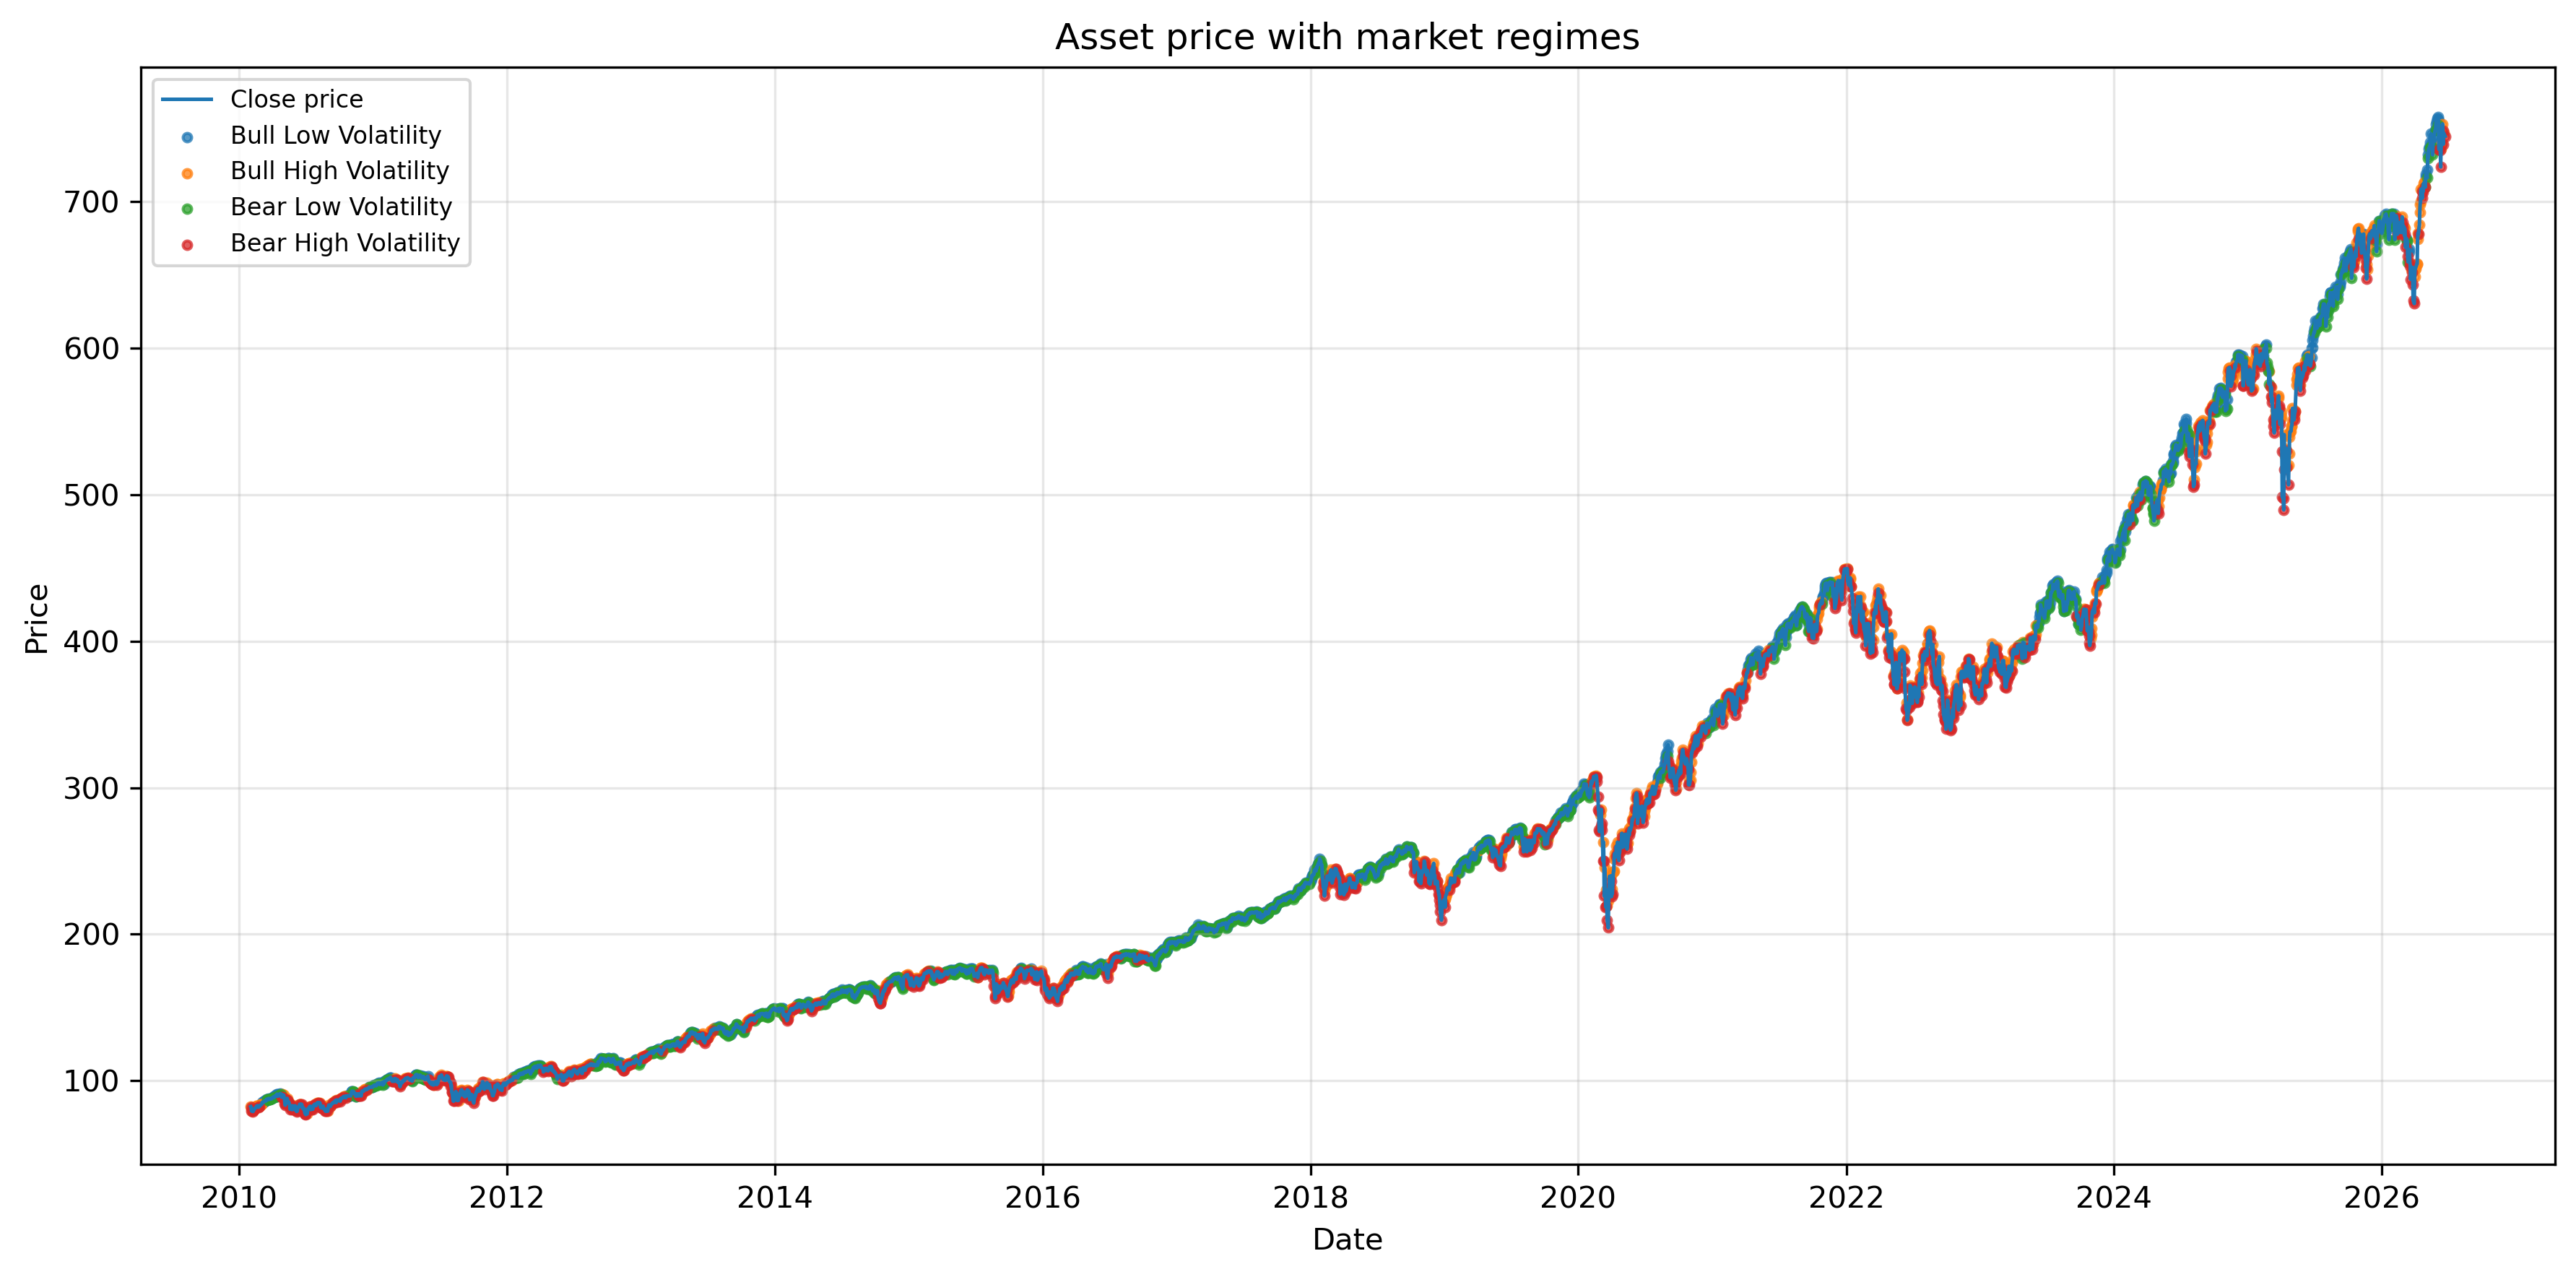
\includegraphics[width=0.95\textwidth]{regimes_over_time.png}
\caption{Asset price with observable regime classification.}
\label{fig:regimes}
\end{figure}

\begin{figure}[H]
\centering
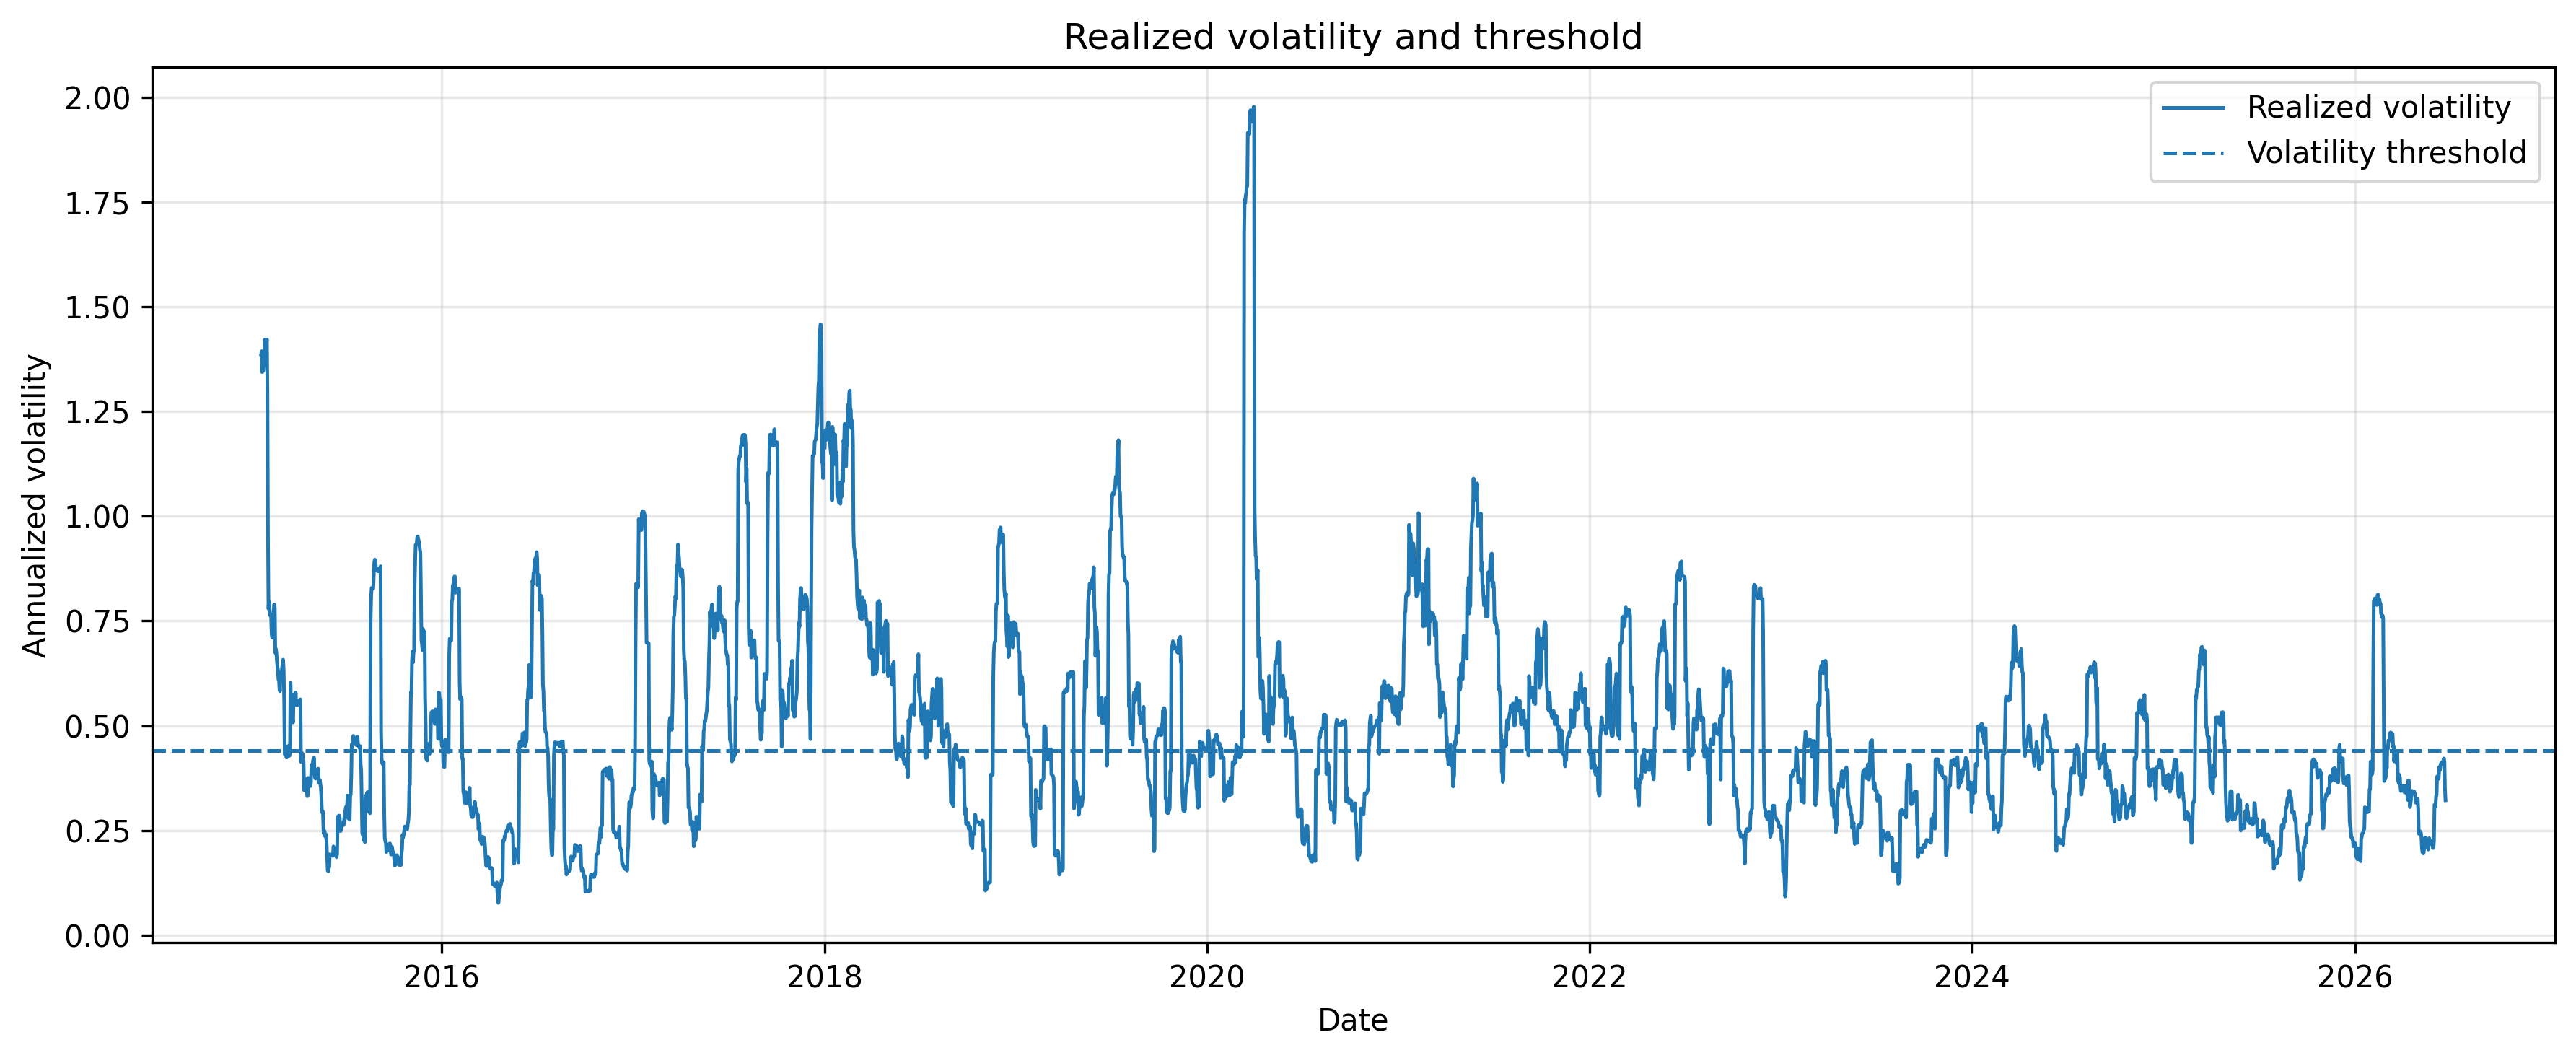
\includegraphics[width=0.95\textwidth]{volatility_threshold.png}
\caption{Rolling realized volatility and volatility threshold.}
\label{fig:volatility}
\end{figure}

% ============================================================
\section{Estimated Markov dynamics}
% ============================================================

Figure \ref{fig:transition-heatmap} displays the estimated transition matrix. The diagonal terms are especially important because they measure regime persistence.

\begin{figure}[H]
\centering
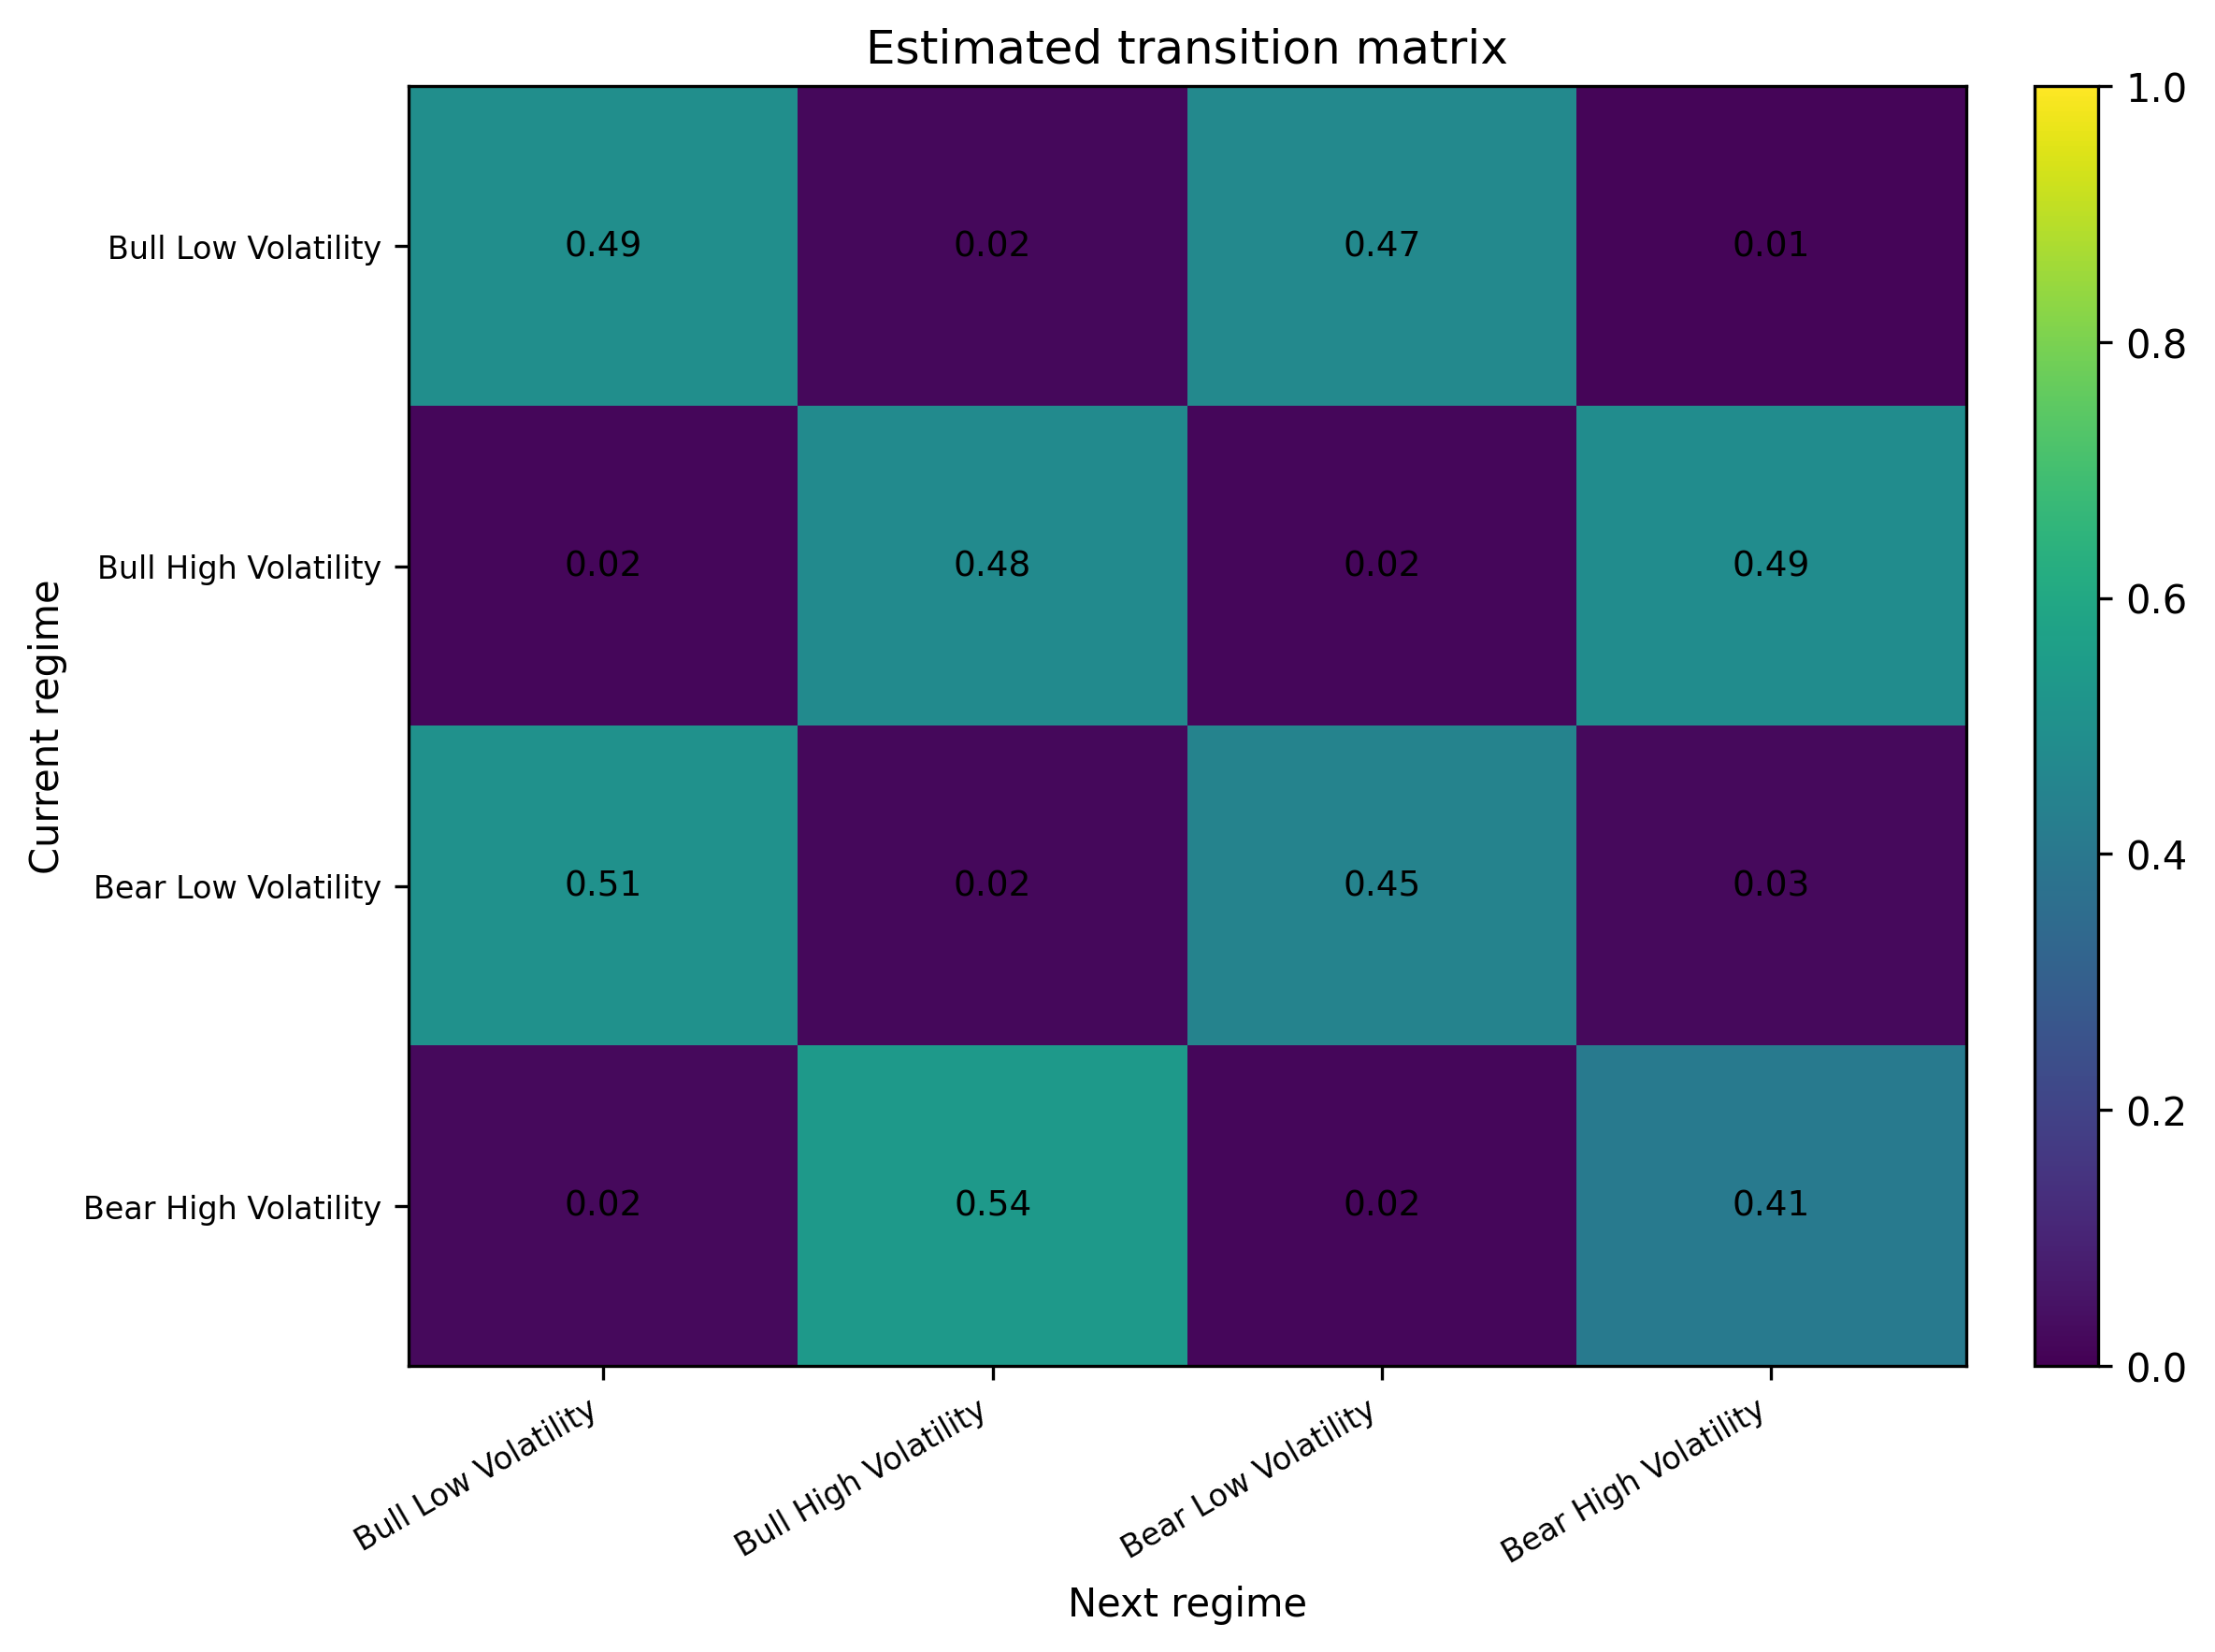
\includegraphics[width=0.82\textwidth]{transition_matrix_heatmap.png}
\caption{Heatmap of the estimated transition matrix.}
\label{fig:transition-heatmap}
\end{figure}

Table \ref{tab:markov-summary} summarizes the estimated Markov chain.

\begin{table}[H]
\centering
\caption{Markov chain summary}
\label{tab:markov-summary}
\begin{tabular}{lcccc}
\toprule
Regime & Persistence & Expected duration & Stationary probability & Outgoing transitions \
\midrule
Bull Low Volatility  & 0.5398 & 2.17 & 0.2832 & 1167 \
Bull High Volatility & 0.5244 & 2.10 & 0.2733 & 1127 \
Bear Low Volatility  & 0.4076 & 1.69 & 0.2167 & 893 \
Bear High Volatility & 0.4244 & 1.74 & 0.2267 & 933 \
\bottomrule
\end{tabular}
\end{table}

The Bull Low Volatility and Bull High Volatility regimes are the most persistent, with diagonal transition probabilities of 0.5398 and 0.5244. The Bear regimes are less persistent, with expected durations below two trading days. This suggests that the regime classification captures some persistence, but not extremely long-lasting states.

The likelihood of the first-order Markov model can be compared to an independent-regime benchmark. The results are:
[
\ell_{\text{Markov}} = -3398.70,
\qquad
\ell_{\text{Independent}} = -5684.30,
]
which gives the likelihood ratio statistic
[
LR = 4571.19.
]
This indicates that conditioning on the current regime substantially improves the fit relative to an independent-regime model.

% ============================================================
\section{Regime-based allocation}
% ============================================================

I now test a simple allocation rule based on the previous day's regime. Let $a_t \in [0,1]$ denote the fraction of the portfolio invested in the risky asset during day $t$. To avoid look-ahead bias, the allocation for day $t$ depends only on the regime observed at day $t-1$.

The baseline allocation rule is reported in Table \ref{tab:allocation-rule}.

\begin{table}[H]
\centering
\caption{Baseline regime-based allocation rule}
\label{tab:allocation-rule}
\begin{tabular}{lc}
\toprule
Previous regime & Allocation \
\midrule
Bull Low Volatility  & 100% \
Bull High Volatility & 75% \
Bear Low Volatility  & 50% \
Bear High Volatility & 0% \
\bottomrule
\end{tabular}
\end{table}

Assuming a zero daily cash return, the gross strategy log-return is approximated by
\begin{equation}
r_t^{\text{strat}}
=
a_t r_t.
\end{equation}

Transaction costs are applied to allocation turnover. If $c_{\text{tc}}$ denotes the proportional transaction cost, the net return is approximated by
\begin{equation}
r_t^{\text{net}}
=
a_t r_t
-
c_{\text{tc}} |a_t-a_{t-1}|.
\end{equation}

In the empirical implementation, transaction costs are set to 5 basis points.

% ============================================================
\section{Backtest results}
% ============================================================

Table \ref{tab:performance} compares the buy-and-hold benchmark, the gross regime strategy, and the net regime strategy after transaction costs.

\begin{table}[H]
\centering
\caption{Backtest performance comparison}
\label{tab:performance}
\begin{tabular}{lcccccc}
\toprule
Strategy & Total return & CAGR & Ann. vol. & Sharpe & Max drawdown & Turnover \
\midrule
Buy and Hold        & 803.80% & 14.41% & 17.17% & 0.79 & -33.72% & -- \
Regime Strategy     & 154.82% & 5.89%  & 9.54%  & 0.60 & -22.07% & 1323.75 \
Regime Strategy Net & 31.46%  & 1.69%  & 9.55%  & 0.18 & -23.82% & 1323.75 \
\bottomrule
\end{tabular}
\end{table}

The gross regime strategy reduces annualized volatility from 17.17% to 9.54% and reduces maximum drawdown from -33.72% to -22.07%. However, it gives up a large share of the upside. The buy-and-hold benchmark strongly outperforms the regime strategy in total return and CAGR.

After transaction costs, performance deteriorates significantly. The net regime strategy has a CAGR of only 1.69%, compared to 5.89% before costs. This is mainly due to high turnover. The result is useful because it shows a realistic limitation: regime information may help reduce risk, but the allocation rule must avoid excessive trading.

Figures \ref{fig:performance} and \ref{fig:drawdowns} show cumulative performance and drawdowns.

\begin{figure}[H]
\centering
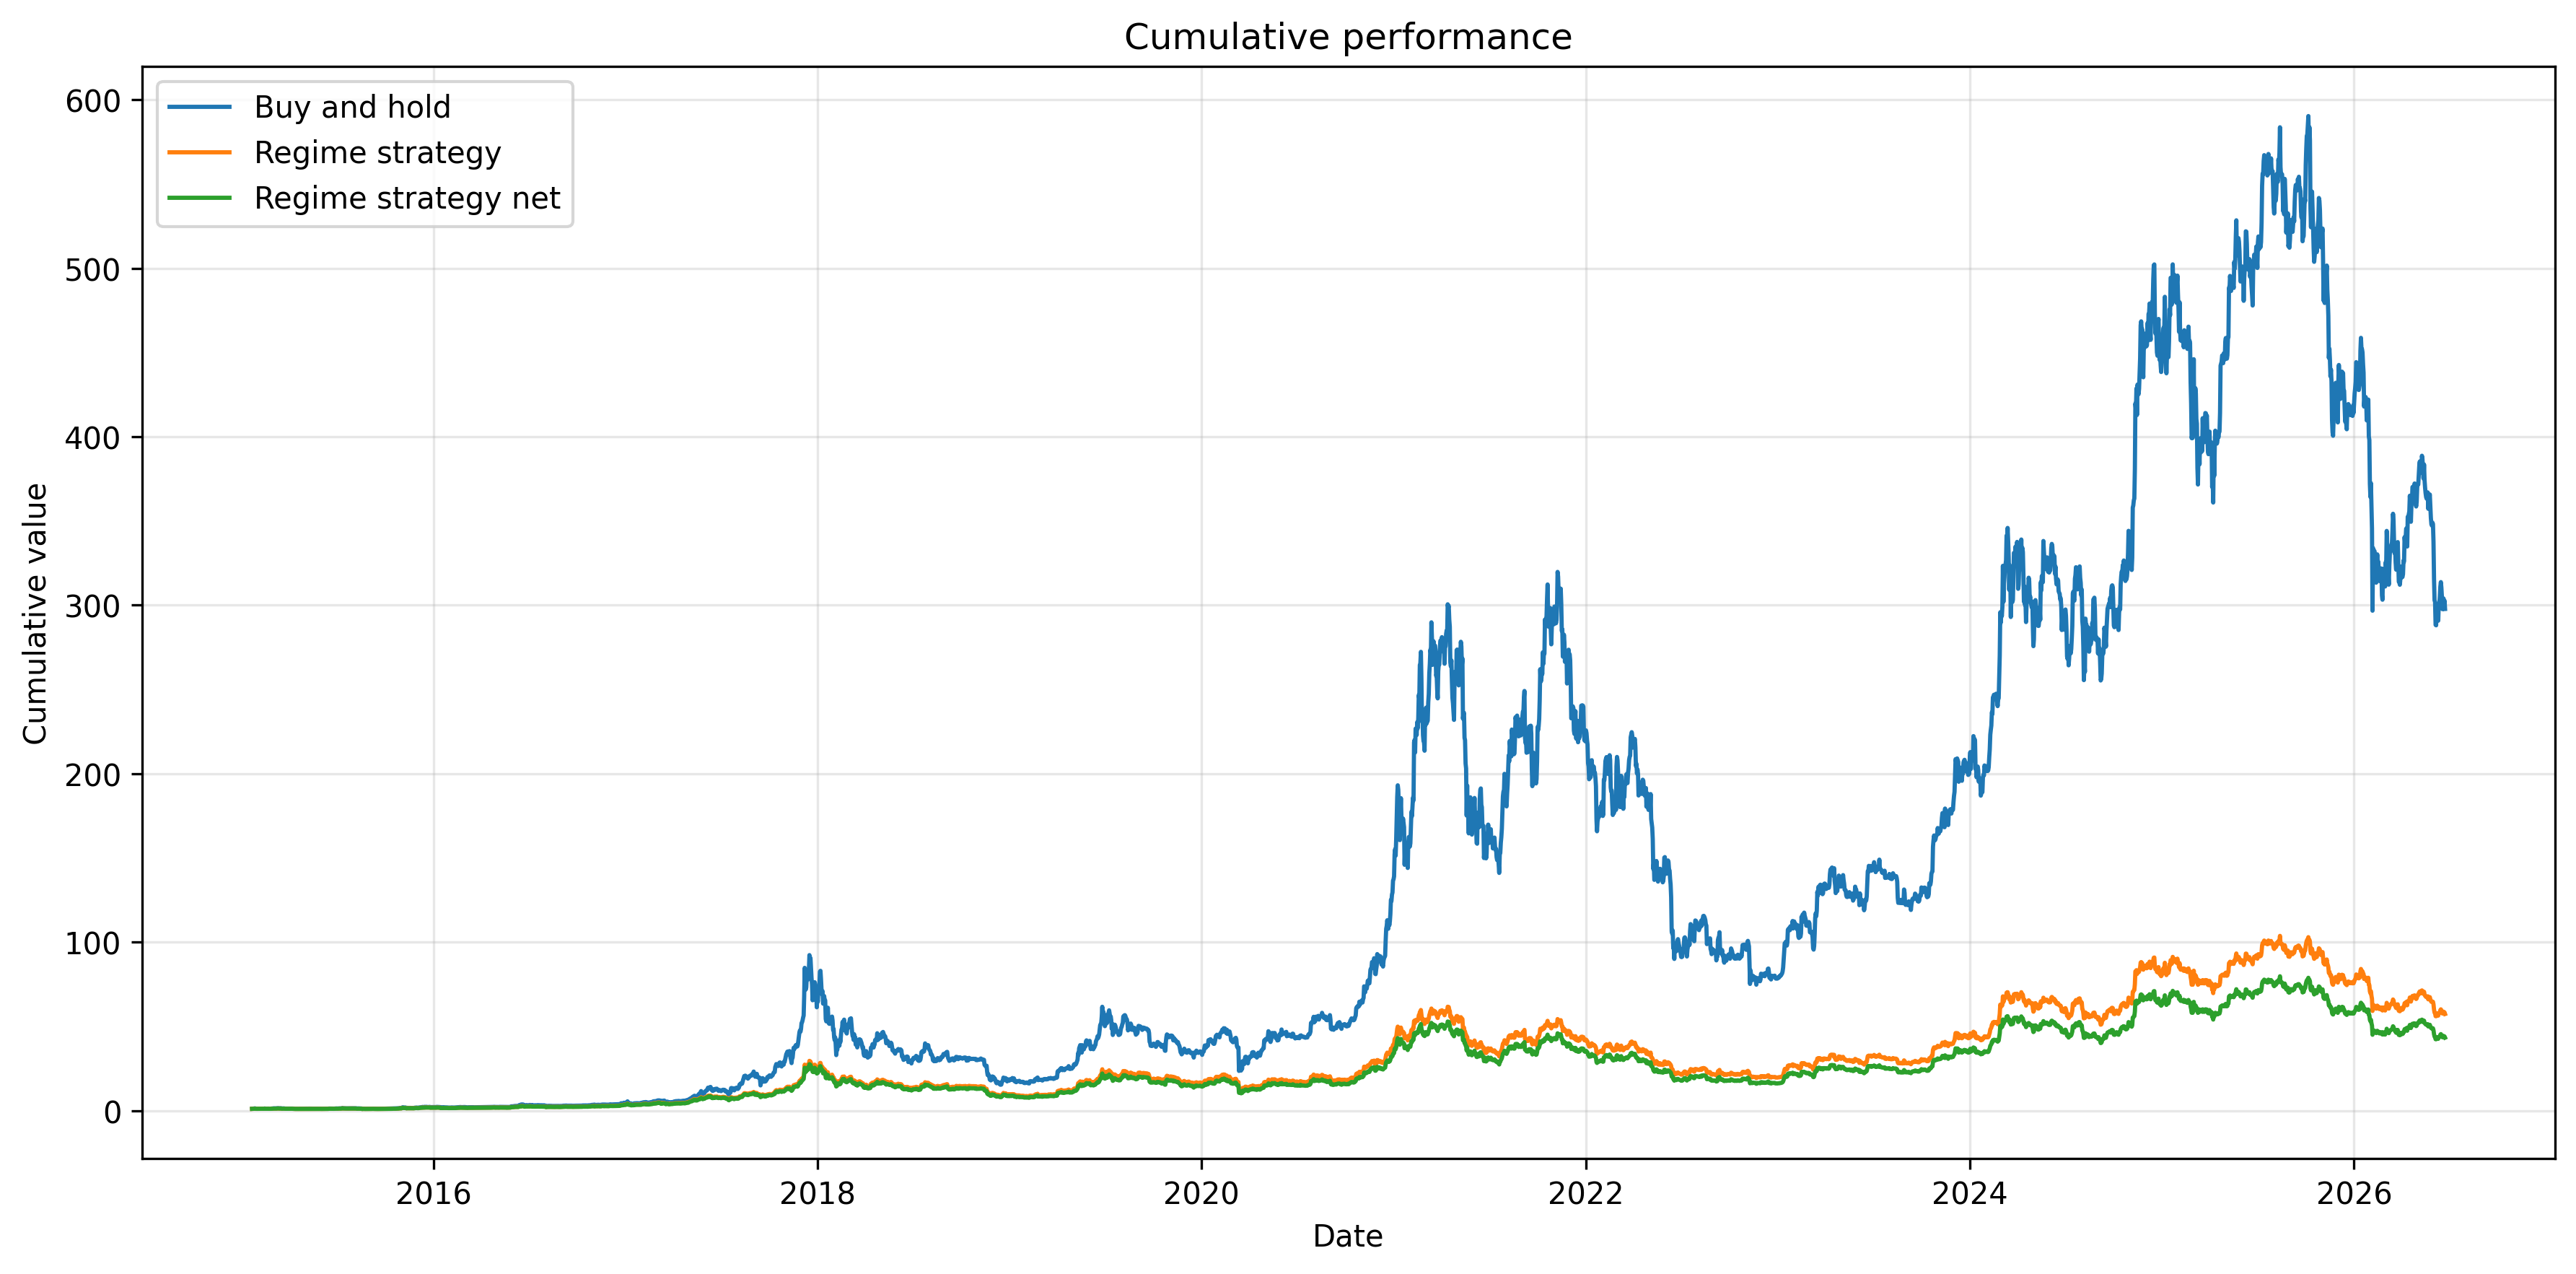
\includegraphics[width=0.95\textwidth]{strategy_vs_benchmark.png}
\caption{Cumulative performance of buy-and-hold and regime-based strategies.}
\label{fig:performance}
\end{figure}

\begin{figure}[H]
\centering
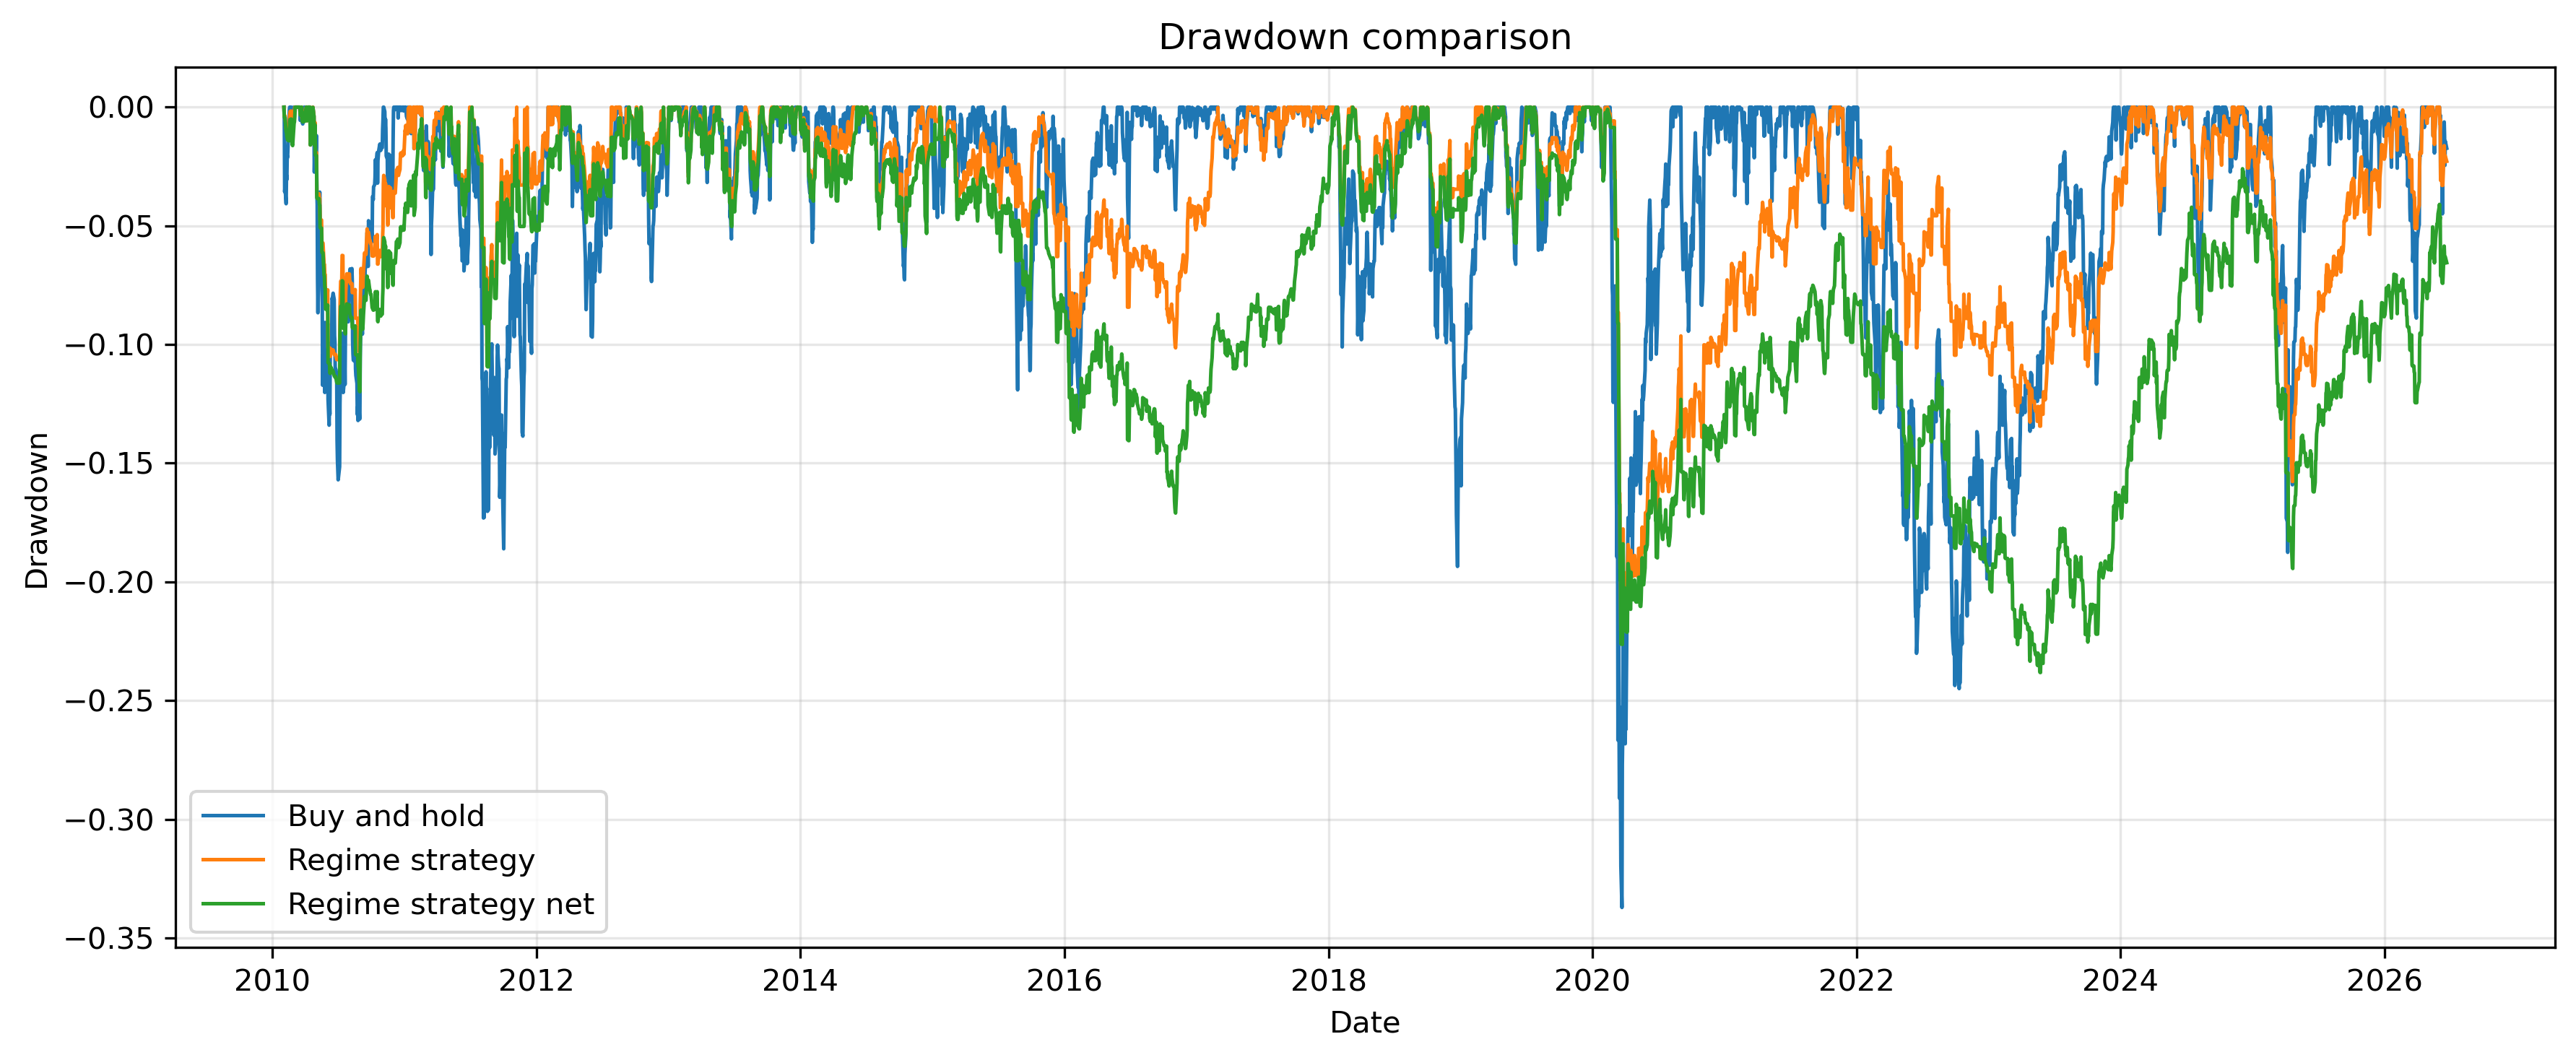
\includegraphics[width=0.95\textwidth]{drawdown_comparison.png}
\caption{Drawdown comparison.}
\label{fig:drawdowns}
\end{figure}

% ============================================================
\section{Limitations and extensions}
% ============================================================

This project should be understood as a clean and interpretable baseline rather than a production-ready investment strategy.

First, the regime classification is based on simple thresholds. This is transparent, but it is also arbitrary. A more advanced project could use quantile thresholds, clustering, Gaussian mixture models, or Hidden Markov Models.

Second, the Markov assumption is restrictive. The next regime may depend not only on the current regime, but also on the duration already spent in that regime, macroeconomic variables, interest rates, liquidity conditions, or volatility indices.

Third, the transition matrix is estimated on the full sample and assumed constant over time. A natural extension would be to estimate rolling transition matrices and study whether regime dynamics change across market environments.

Fourth, the allocation rule is heuristic. It is useful as a baseline, but it is not derived from a formal optimization problem. A more rigorous version could estimate regime-conditional expected returns and variances, then choose exposure through a mean-variance or expected-utility criterion.

Finally, the backtest highlights the importance of transaction costs. A regime-based allocation rule can reduce risk, but if it changes exposure too frequently, its performance may be strongly reduced after costs.

% ============================================================
\section{Conclusion}
% ============================================================

This report developed a transparent Markov chain framework for analysing observable market regimes. Starting from daily prices, I computed log-returns and realized volatility, classified each trading day into one of four interpretable regimes, and estimated the transition matrix of the resulting Markov chain.

The empirical application to SPY shows meaningful regime persistence. The Markov model fits the regime sequence much better than an independent-regime benchmark. The estimated transition matrix also provides intuitive measures of persistence, expected duration, and long-run regime frequencies.

The regime-based allocation strategy reduces volatility and drawdowns relative to buy-and-hold. However, it also sacrifices a large part of the upside, and transaction costs significantly reduce performance because the strategy generates high turnover.

The main value of the project is therefore not to propose a ready-to-trade strategy. Its value is to provide a reproducible quantitative finance baseline connecting probability theory, financial time series, Markov chains, and disciplined backtesting. It also provides a natural starting point for more advanced extensions such as rolling transition matrices, clustering-based regimes, Hidden Markov Models, and regime-conditional portfolio optimization.

% ============================================================
\begin{thebibliography}{9}

\bibitem{hamilton1989}
Hamilton, J. D. (1989).
A new approach to the economic analysis of nonstationary time series and the business cycle.
\emph{Econometrica}, 57(2), 357--384.

\bibitem{rabiner1989}
Rabiner, L. R. (1989).
A tutorial on Hidden Markov Models and selected applications in speech recognition.
\emph{Proceedings of the IEEE}, 77(2), 257--286.

\bibitem{tsay2010}
Tsay, R. S. (2010).
\emph{Analysis of Financial Time Series}.
Wiley.

\bibitem{cont2001}
Cont, R. (2001).
Empirical properties of asset returns: stylized facts and statistical issues.
\emph{Quantitative Finance}, 1(2), 223--236.

\end{thebibliography}

\end{document}
